


\tikzset{every picture/.style={line width=0.75pt}} %set default line width to 0.75pt        

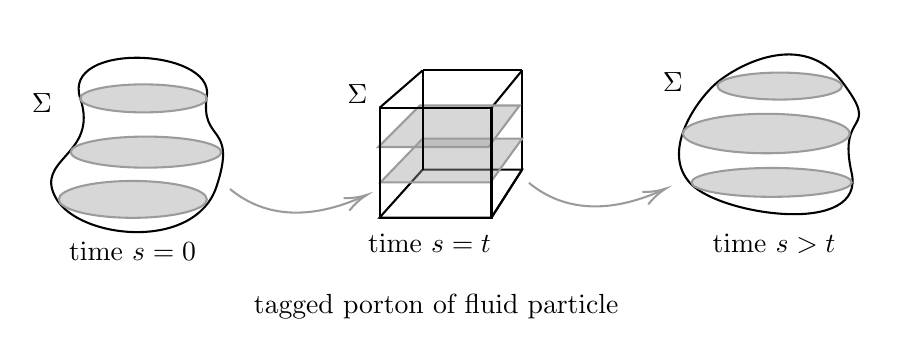
\begin{tikzpicture}[x=0.75pt,y=0.75pt,yscale=-1,xscale=1]
%uncomment if require: \path (0,153); %set diagram left start at 0, and has height of 153

%Shape: Polygon Curved [id:ds5674727895312841] 
\draw   (104.84,28.32) .. controls (95.63,0.69) and (169.29,4.15) .. (165.84,27.17) .. controls (162.38,50.18) and (180.8,39.9) .. (170.44,70.9) .. controls (160.08,101.9) and (104.84,96.22) .. (93.33,76.73) .. controls (81.82,57.23) and (114.05,55.94) .. (104.84,28.32) -- cycle ;
%Shape: Ellipse [id:dp04402872664839763] 
\draw  [color={rgb, 255:red, 155; green, 155; blue, 155 }  ,draw opacity=1 ][fill={rgb, 255:red, 155; green, 155; blue, 155 }  ,fill opacity=0.4 ] (100.24,54.21) .. controls (100.24,50.08) and (116.47,46.73) .. (136.49,46.73) .. controls (156.51,46.73) and (172.74,50.08) .. (172.74,54.21) .. controls (172.74,58.34) and (156.51,61.69) .. (136.49,61.69) .. controls (116.47,61.69) and (100.24,58.34) .. (100.24,54.21) -- cycle ;
%Shape: Ellipse [id:dp05017881529269319] 
\draw  [color={rgb, 255:red, 155; green, 155; blue, 155 }  ,draw opacity=1 ][fill={rgb, 255:red, 155; green, 155; blue, 155 }  ,fill opacity=0.4 ] (94.48,76.98) .. controls (94.48,72.07) and (110.45,68.1) .. (130.16,68.1) .. controls (149.86,68.1) and (165.84,72.07) .. (165.84,76.98) .. controls (165.84,81.89) and (149.86,85.86) .. (130.16,85.86) .. controls (110.45,85.86) and (94.48,81.89) .. (94.48,76.98) -- cycle ;
%Shape: Ellipse [id:dp9015870670707791] 
\draw  [color={rgb, 255:red, 155; green, 155; blue, 155 }  ,draw opacity=1 ][fill={rgb, 255:red, 155; green, 155; blue, 155 }  ,fill opacity=0.4 ] (104.84,28.32) .. controls (104.84,24.59) and (118.49,21.57) .. (135.34,21.57) .. controls (152.18,21.57) and (165.84,24.59) .. (165.84,28.32) .. controls (165.84,32.04) and (152.18,35.06) .. (135.34,35.06) .. controls (118.49,35.06) and (104.84,32.04) .. (104.84,28.32) -- cycle ;
%Straight Lines [id:da09945186129015027] 
\draw    (302.96,85.75) -- (317.73,62.61) ;
%Straight Lines [id:da711160596750477] 
\draw    (317.73,62.61) -- (317.73,14.82) ;
%Straight Lines [id:da15820533408851523] 
\draw    (302.96,32.84) -- (317.73,14.82) ;
%Straight Lines [id:da29785535615300107] 
\draw    (249.04,32.84) -- (269.81,14.82) ;
%Straight Lines [id:da8060543139467564] 
\draw    (269.81,14.82) -- (317.73,14.82) ;
%Shape: Polygon Curved [id:ds9769011976202862] 
\draw   (410.84,21.39) .. controls (420.5,12.82) and (452.5,-5.25) .. (471.84,20.24) .. controls (491.18,45.72) and (469.38,33.12) .. (476.44,63.97) .. controls (483.5,94.82) and (414.5,84.82) .. (399.33,69.8) .. controls (384.16,54.77) and (401.18,29.95) .. (410.84,21.39) -- cycle ;
%Shape: Ellipse [id:dp7706483204857539] 
\draw  [color={rgb, 255:red, 155; green, 155; blue, 155 }  ,draw opacity=1 ][fill={rgb, 255:red, 155; green, 155; blue, 155 }  ,fill opacity=0.4 ] (395.24,45.25) .. controls (395.24,40) and (413.2,35.75) .. (435.37,35.75) .. controls (457.53,35.75) and (475.5,40) .. (475.5,45.25) .. controls (475.5,50.5) and (457.53,54.75) .. (435.37,54.75) .. controls (413.2,54.75) and (395.24,50.5) .. (395.24,45.25) -- cycle ;
%Shape: Ellipse [id:dp3360158695617945] 
\draw  [color={rgb, 255:red, 155; green, 155; blue, 155 }  ,draw opacity=1 ][fill={rgb, 255:red, 155; green, 155; blue, 155 }  ,fill opacity=0.4 ] (399.33,68.8) .. controls (399.33,64.96) and (416.61,61.84) .. (437.92,61.84) .. controls (459.22,61.84) and (476.5,64.96) .. (476.5,68.8) .. controls (476.5,72.64) and (459.22,75.75) .. (437.92,75.75) .. controls (416.61,75.75) and (399.33,72.64) .. (399.33,68.8) -- cycle ;
%Shape: Ellipse [id:dp4350222330863558] 
\draw  [color={rgb, 255:red, 155; green, 155; blue, 155 }  ,draw opacity=1 ][fill={rgb, 255:red, 155; green, 155; blue, 155 }  ,fill opacity=0.4 ] (411.84,22.39) .. controls (411.84,18.8) and (425.27,15.89) .. (441.84,15.89) .. controls (458.41,15.89) and (471.84,18.8) .. (471.84,22.39) .. controls (471.84,25.98) and (458.41,28.89) .. (441.84,28.89) .. controls (425.27,28.89) and (411.84,25.98) .. (411.84,22.39) -- cycle ;
%Shape: Polygon [id:ds08380318600800352] 
\draw   (269.81,62.61) -- (317.73,62.61) -- (302.96,85.75) -- (249.04,85.75) -- cycle ;
%Shape: Polygon [id:ds30480330695766544] 
\draw  [color={rgb, 255:red, 155; green, 155; blue, 155 }  ,draw opacity=1 ][fill={rgb, 255:red, 155; green, 155; blue, 155 }  ,fill opacity=0.4 ] (269.81,47.71) -- (317.73,47.71) -- (302.5,68.75) -- (249.5,68.75) -- cycle ;
%Shape: Polygon [id:ds7937950735293224] 
\draw  [color={rgb, 255:red, 155; green, 155; blue, 155 }  ,draw opacity=1 ][fill={rgb, 255:red, 155; green, 155; blue, 155 }  ,fill opacity=0.4 ] (268.5,31.75) -- (316.5,31.75) -- (301.5,51.75) -- (290,51.75) -- (248.5,51.75) -- cycle ;
%Straight Lines [id:da9621822973654746] 
\draw    (269.81,14.82) -- (269.81,62.61) ;
%Shape: Rectangle [id:dp058361048141616134] 
\draw  [color={rgb, 255:red, 0; green, 0; blue, 0 }  ,draw opacity=1 ] (249.04,32.84) -- (302.96,32.84) -- (302.96,85.75) -- (249.04,85.75) -- cycle ;
%Curve Lines [id:da8858304884140866] 
\draw [color={rgb, 255:red, 155; green, 155; blue, 155 }  ,draw opacity=1 ]   (177,72) .. controls (189.81,82.59) and (210.37,89.54) .. (241.57,75.41) ;
\draw [shift={(243,74.75)}, rotate = 154.89] [color={rgb, 255:red, 155; green, 155; blue, 155 }  ,draw opacity=1 ][line width=0.75]    (10.93,-3.29) .. controls (6.95,-1.4) and (3.31,-0.3) .. (0,0) .. controls (3.31,0.3) and (6.95,1.4) .. (10.93,3.29)   ;
%Curve Lines [id:da6710279850520793] 
\draw [color={rgb, 255:red, 155; green, 155; blue, 155 }  ,draw opacity=1 ]   (321,69) .. controls (333.81,79.59) and (354.37,86.54) .. (385.57,72.41) ;
\draw [shift={(387,71.75)}, rotate = 154.89] [color={rgb, 255:red, 155; green, 155; blue, 155 }  ,draw opacity=1 ][line width=0.75]    (10.93,-3.29) .. controls (6.95,-1.4) and (3.31,-0.3) .. (0,0) .. controls (3.31,0.3) and (6.95,1.4) .. (10.93,3.29)   ;

% Text Node
\draw (80,24.4) node [anchor=north west][inner sep=0.75pt]    {$\Sigma $};
% Text Node
\draw (232,20.4) node [anchor=north west][inner sep=0.75pt]    {$\Sigma $};
% Text Node
\draw (384,14.4) node [anchor=north west][inner sep=0.75pt]    {$\Sigma $};
% Text Node
\draw (98,96) node [anchor=north west][inner sep=0.75pt]   [align=left] {time $\displaystyle s=0$};
% Text Node
\draw (242,92) node [anchor=north west][inner sep=0.75pt]   [align=left] {time $\displaystyle s=t$};
% Text Node
\draw (408,92) node [anchor=north west][inner sep=0.75pt]   [align=left] {time $\displaystyle s >t$};
% Text Node
\draw (187,121) node [anchor=north west][inner sep=0.75pt]   [align=left] {tagged porton of fluid particle};


\end{tikzpicture}
